% !TEX root = ../../../main.tex

% Bibtex

%https://pixabay.com/photos/shoe-shoe-rack-rack-black-and-white-1099446/
% https://www2.htw-dresden.de/~sobe/Vorjahre/Vo_InfoMB_Jg11/7_Datenstrukturen.pdf

\toggletrue{image}
\toggletrue{imagehover}
\chapterimage{donald_knuth}
\chapterimagetitle{\uppercase{Donal Knuth}}
\chapterimageurl{https://xkcd.com/163/}
\chapterimagehover{His books were kinda intimidating; rappelling down through his skylight seemed like the best option.}

\chapter{Einführung in Datenstrukturen}
\label{chapter-einfuehrung-datenstrukturen}

Algorithmen verarbeiten Daten, um Probleme zu lösen. Dabei ist es sinnvoll, die Daten so zu strukturieren, dass der Algorithmus die Verarbeitung effizient durchführen kann.

\section{Beispiele für eine Datenstruktur aus dem Alltag}

\begin{example}
Das Ordnen von Gegenständen kennen wir auch aus dem Alltag. Zum Beispiel können Sie Schuhe in einem Schuhregal in Fächer einordnen. Das erleichtert (hoffentlich) die Suche nach einem bestimmten Paar Schuhe.
\end{example}

\begin{figure}[htb]
	\centering
	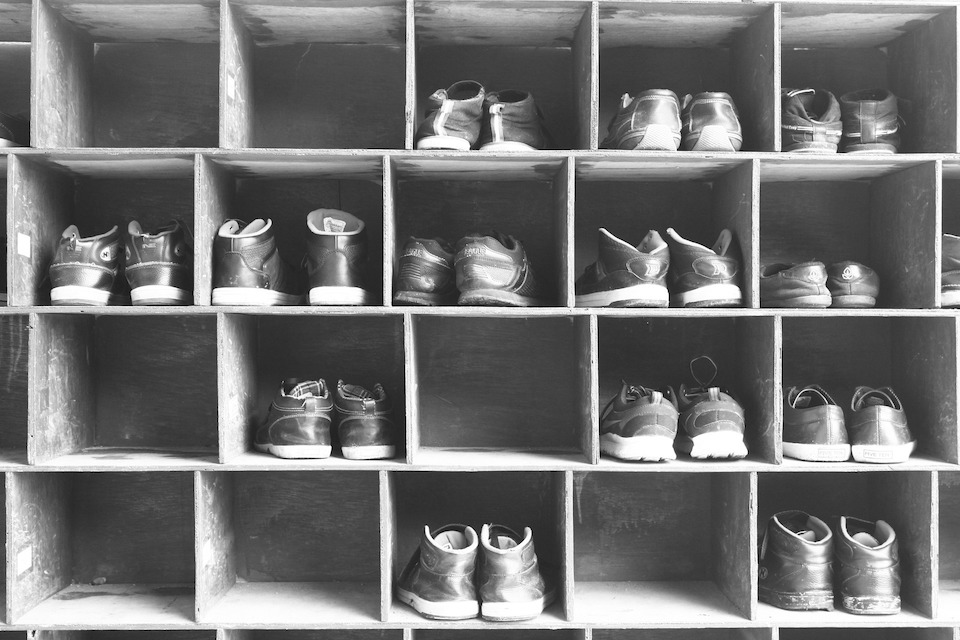
\includegraphics[scale=0.2]{schuhregal}
\end{figure}

\begin{figure}[htb]
	\centering
	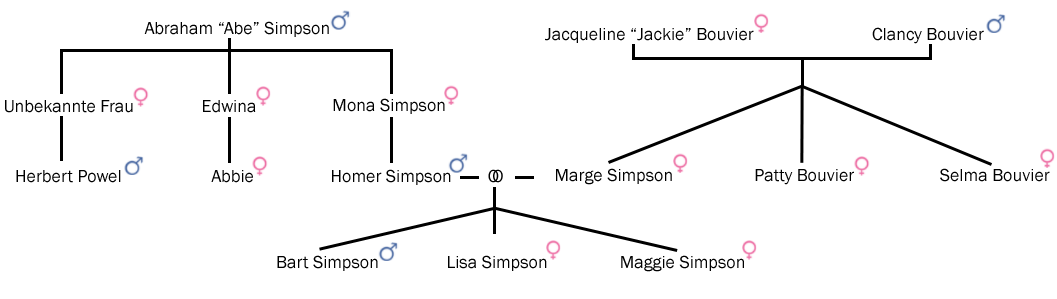
\includegraphics[scale=0.3]{stammbaum_simpsons}
\end{figure}

\begin{example}
Auch ein Stammbaum ist eine Datenstruktur des täglichen Lebens. Wir ordnen die Namen der Familienmitglieder so an, dass Vorfahren und Nachkommen leicht zu erkennen sind.
\end{example}

Die Lernziele für dieses Kapitel sind:

\newcommand{\einfuehrungDatenstrukturenLernziele}{
\protect\begin{todolist}
\item Sie erklären die Idee einer Datenstruktur anhand eines alltäglichen Beispiels.
\item Sie definieren, was wir in der Informatik unter einer Datenstruktur verstehen.
\item Sie erläutern die Datenstruktur Array.
\end{todolist}
}

\lernziel{\autoref{chapter-einfuehrung-datenstrukturen}, \nameref{chapter-einfuehrung-datenstrukturen}}{\protect\einfuehrungDatenstrukturenLernziele}

\einfuehrungDatenstrukturenLernziele

\section{Was ist eine Datenstruktur im Sinne der Informatik?}

Beim Entwurf von Algorithmen spielt die Wahl der Datenstrukturen eine zentrale Rolle.

\begin{definition}[Datenstruktur]
Eine Datenstruktur bestimmt, wie Daten \textbf{organisiert} und \textbf{verwaltet} werden, um die Effizienz von Algorithmen zu verbessern. Jede Datenstruktur kann Daten auf unterschiedliche Weise speichern. Durch die spezielle \textbf{Anordnung der Daten} versuchen wir, die \textbf{Verarbeitung der Daten} zu \textbf{optimieren}. Meistens optimieren wir entweder den für die Daten benötigten \textbf{Speicherplatz} oder die \textbf{Ausführungsgeschwindigkeit}.
\end{definition}

\begin{example}
Eine Datenstruktur kann beispielsweise ein Array, eine Liste, ein Baum, ein Stapel oder eine Warteschlange sein.
\end{example}

Mit der richtigen Datenstruktur können Algorithmen schneller und effizienter arbeiten. Datenstrukturen spielen daher eine wichtige Rolle bei der Entwicklung von Algorithmen und der Lösung von Problemen in der Informatik.

\section{Arrays}

Ein Array (dt. Feld) ist eine der grundlegendsten Datenstrukturen.

\begin{definition}[Array]
	Ein Array ist eine \textbf{geordnete Sammlung} von Elementen desselben Typs. Die \textbf{Anzahl der Elemente} muss bei der Erstellung des Arrays \textbf{festgelegt} werden und kann \textbf{nicht mehr geändert} werden. Ein \textbf{Element} kann in einem Array \textbf{mehrfach} vorkommen. Jedes Element im Array hat einen \textbf{Index}, der angibt, an welcher \textbf{Position im Array} es sich befindet. Dies ermöglicht einen schnellen Zugriff auf ein Element im Array.
\end{definition}

Wir notieren ein Array in \textbf{eckigen Klammern} und trennen die \textbf{Elemente} durch Kommas. Hat ein Array $n$ Elemente, so hat das \textbf{erste Element den Index $0$} und das \textbf{letzte Element den Index $n-1$}.

\begin{example}
Das Array \lstinline[language=pseudocode]{[2, 4, 10, 5, -15, 13, 10]} hat \textbf{7 Elemente}. Jedes Element ist \textbf{eine Ganzzahl}. Der \textbf{Index} bestimmt, an welcher \textbf{Position im Array} das Element gespeichert ist. Die folgende Tabelle zeigt das Array mit den zugehörigen Indizes (Plural von Index).

\begin{table}[htb]
\centering
\begin{tblr}{
    colspec = {cccccccc},
    vline{2-Z} = {1}{solid}
}
\cline{2-8}
Element & 2 & 4 & 10 & 5 & -15 & 13 & 10 \\
\cline{2-8}
Index   & 0 & 1 & 2 & 3 & 4 & 5 & 6\\
\end{tblr}
\end{table}
\end{example}

\subsection{Zugriff auf Array-Elemente}

Über den \textbf{Index} können wir auf ein Element innerhalb des Arrays \textbf{zugreifen}. Wir können dann zum Beispiel einen Vergleich oder eine Berechnung mit dem Element durchführen. Der Zugriff auf ein \textbf{Array-Element} verändert das Array \textbf{nicht}. Die \textbf{eckigen Klammern} werden auch verwendet, um auf ein Array-Element zuzugreifen.

\begin{example}
Der folgende Pseudocode zeigt den Umgang mit einem Array, Indizes, Variablen und der Addition. In Zeile 4 und 5 wird die Zahl aus dem Array kopiert, \textbf{nicht} verschoben.
\begin{lstlisting}[language=pseudocode, caption={Die ersten beiden Zahlen des Arrays werden addiert.}, label={lst-array-examples-1}]
# Die Variable A speichert das Array mit 7 Zahlen.
A $\gets$ [2, 4, 10, 5, -15, 13, 10]

x $\gets$ A[0]
y $\gets$ A[1]
summe $\gets$ x + y
output: summe
\end{lstlisting}
\end{example}

\subsection{Ausgewählte Probleme zum Einstieg}

Ein Array erlaubt uns nun, vielfältigere Probleme zu betrachten.

\begin{problem}[Maximum-n-Zahlen]\label{problem-max-n-zahlen}
Es sind $n$ Zahlen in einem Array $A$ gegeben. Es soll das \textbf{Maximum} (die grösste Zahl) ausgegeben werden.
\end{problem}

Da wir für das Problem \autoref{problem-max-n-zahlen} nicht wissen, wie viele Zahlen im Array gespeichert sind, müssen wir den Algorithmus so formulieren, dass er für eine beliebige Anzahl von Zahlen funktioniert. Dies erreichen wir mithilfe einer Schleife. \autoref{lst-algo-max-n-zahlen} zeigt den Algorithmus für das Problem \autoref{problem-max-n-zahlen}.

\begin{lstlisting}[language=pseudocode, caption={In Zeile \num{5} greifen wir auf das Array zu und kopieren die Zahl aus dem Array mit dem Index \lstinline{i} in die Variable \lstinline{zahl}.}, label={lst-algo-max-n-zahlen}]
input: Ein Array A mit n Zahlen.
maximum $\gets$ unbekannt
i $\gets$ 0
# In der Schleife werden alle Zahlen des Arrays überprüft
# Über den Index wird eine Zahl nach der anderen betrachtet
loop as long as i < n {
 zahl $\gets$ A[i]
 if maximum ist unbekannt oder maximum < zahl {
  maximum $\gets$ zahl
 }
 Erhöhe i um 1
}
output: maximum
\end{lstlisting}

Wir können natürlich auch eine Berechnung mit den Zahlen des Arrays durchführen.

\begin{problem}[Addition-n-Zahlen]\label{problem-addition-n-zahlen}
	Es sind $n$ Zahlen in einem Array $A$ gegeben. Es soll die \textbf{Summe} der $n$ Zahlen berechnet und ausgegeben werden.
\end{problem}

Der Computer kann \textbf{nicht} alle Zahlen in einem Berechnungsschritt addieren. Es können maximal zwei Zahlen pro Berechnungsschritt addiert werden. Der Algorithmus in \autoref{lst-algo-addition-n-zahlen} berücksichtigt diese Einschränkung.

\begin{lstlisting}[language=pseudocode, caption={Wir verwenden die Variable \lstinline{summe}, um die Zahlen fortlaufend zu addieren.}, label={lst-algo-addition-n-zahlen}]
input: Ein Array A mit n Zahlen.
summe $\gets$ 0
i $\gets$ 0
loop as long as i < n {
 # Diese Zeile wird von rechts nach links abgearbeitet.
 # Der Inhalt der Variablen summe wird überschrieben.
 summe $\gets$ summe + A[i]
 Erhöhe i um 1
}
output: summe
\end{lstlisting}

Wenn wir mit einem Array arbeiten und jede Zahl in diesem Array nacheinander verarbeiten wollen, dann können wir immer das Prinzip aus \autoref{lst-algo-max-n-zahlen} bzw. \autoref{lst-algo-addition-n-zahlen} verwenden.

\begin{hinweis}
Wir beschränken uns hier auf Arrays, die ausschliesslich natürliche Zahlen speichern. Natürlich können Arrays auch Fliesskommazahlen oder Texte speichern.
\end{hinweis}

\section{Sortierte Arrays}

Ein sortiertes Array ist im Prinzip die gleiche Datenstruktur wie ein Array. Der Unterschied zum Array besteht lediglich darin, dass die \textbf{Elemente} des Arrays \textbf{sortiert} sind.

\begin{definition}[Sortiertes Array]
Ein Array $A$ mit $n$ Elementen ist \textbf{aufsteigend} sortiert, wenn das kleinste Element den Index $0$, das zweitkleinste Element den Index $1$, das drittkleinste Element den Index $2$, $\dots$ und das grösste Element den Index $n-1$ hat. Dann gilt: 
\begin{align*}
A[0] \leq A[1] \leq A[2] \leq \cdots \leq A[n - 2] A\leq A[n - 1]
\end{align*}
Für den umgekehrten Fall sprechen wir von einem \textbf{absteigend} sortierten Array. Dann gilt:
\begin{align*}
A[0] \geq A[1] \geq A[2] \geq \cdots \geq A[n - 2] A\geq A[n - 1]
\end{align*}
Das grösste Element hat dann den Index $0$ und das kleinste Element den Index $n-1$.
\end{definition}

\begin{important}
Arrays besitzen eine \textbf{feste Grösse} (z.B. $n$ Zahlen). Es können \textbf{keine neuen Elemente hinzugefügt} werden.  Wir können aber den \textbf{Inhalt des Arrays verändern}. Wir können also aus einem unsortierten Array ein sortiertes Array erzeugen.
\end{important}

\section{Übungen}

\begin{exercise}
Entwerfen Sie in Pseudocode einen Algorithmus für das folgende Problem.

\begin{problem}[Minimum-n-Zahlen]\label{problem-minimum-n-zahlen}
Es sind $n$ Zahlen in einem Array $A$ gegeben. Es soll das \textbf{Minimum} (die kleinste Zahl) ausgegeben werden.
\end{problem}

\fillwithgrid	{\stretch{1}}
\end{exercise}
\begin{solution}
\begin{minipage}{\linewidth}
\begin{lstlisting}[language=pseudocode, caption={Algorithmus für das Problem \protect\autoref{problem-minimum-n-zahlen}}, label={lst-algo-minimum-n-zahlen}]
input: Ein Array A mit n Zahlen.
minimum $\gets$ unbekannt
i $\gets$ 0
loop as long as i < n {
 zahl $\gets$ A[i]
 if minimum ist unbekannt oder minimum > zahl {
  minimum $\gets$ zahl
 }
 Erhöhe i um 1
}
output: minimum
\end{lstlisting}
\end{minipage}
\end{solution}

\newpage

\begin{exercise}
Entwerfen Sie in Pseudocode einen Algorithmus für das folgende Problem.

\begin{problem}[Durchschnitt-n-Zahlen]\label{problem-durchschnitt-n-zahlen}
Es sind $n$ Zahlen in einem Array $A$ gegeben. Es soll der \textbf{Durchschnitt} der $n$ Zahlen ausgegeben werden.
\end{problem}

\fillwithgrid	{3.5in}
\end{exercise}
\begin{solution}
\begin{minipage}{\linewidth}
\begin{lstlisting}[language=pseudocode, caption={Algorithmus für das Problem \protect\autoref{problem-durchschnitt-n-zahlen}}, label={lst-algo-durchschnitt-n-zahlen}]
input: Ein Array A mit n Zahlen.
summe $\gets$ 0
i $\gets$ 0
loop as long as i < n {
 summe $\gets$ summe + A[i]
 Erhöhe i um 1
}
durchschnitt $\gets$ summe / n
output: durchschnitt
\end{lstlisting}
\end{minipage}
\end{solution}

\begin{exercise}
Entwerfen Sie einen Algorithmus in Pseudocode für folgendes Problem.

\begin{problem}[Anzahl-Minima-n-Zahlen]\label{problem-anzahl-minima-n-zahlen}
	Es sind $n$ Zahlen in einem Array $A$ gegeben. Zahlen können \textbf{mehrfach} vorkommen. Es soll die \textbf{Anzahl der Minima} ausgegeben werden (das heisst, wie oft kommt das Minimum im Array der Zahlen vor).
\end{problem}

\fillwithgrid	{\stretch{1}}
\end{exercise}
\begin{solution}
\begin{minipage}{\linewidth}
\begin{lstlisting}[language=pseudocode, caption={Algorithmus für das Problem \protect\autoref{problem-anzahl-minima-n-zahlen}}, label={lst-algo-anzahl-minima-n-zahlen}]
input: Ein Array A mit n Zahlen.
minimum $\gets$ unbekannt
i $\gets$ 0
loop as long as i < n {
 zahl $\gets$ A[i]
 if minimum ist unbekannt oder minimum > zahl {
  minimum $\gets$ zahl
 }
 Erhöhe i um 1
}
anzahl $\gets$ 0
i $\gets$ 0
loop as long as i < n {
 if minimum = A[i] {
  anzahl $\gets$ anzahl + 1
 }
 Erhöhe i um 1
}
output: minimum, anzahl
\end{lstlisting}
\end{minipage}
\end{solution}

\newpage

\begin{exercise}
Entwerfen Sie in Pseudocode einen Algorithmus für das folgende Problem.

\begin{problem}[Min-Median-Max-n-Zahlen]\label{problem-min-median-max-n-zahlen}
	Es sind $n$ Zahlen in einem \textbf{aufsteigend, sortierten Array} $A$ gegeben. Es sollen das \textbf{Minimum}, das \textbf{Maximum} und der \textbf{Median} der $n$ Zahlen ausgegeben werden.
\end{problem}
\begin{solution}
\begin{minipage}{\linewidth}
\begin{lstlisting}[language=pseudocode, caption={Algorithmus für das Problem \protect\autoref{problem-min-median-max-n-zahlen}}, label={lst-algo-min-median-max-n-zahlen}]
input: Ein Array A mit n Zahlen.
# In einem aufsteigend sortieren Array ist das Minimum 
# die erste Zahl und das Maximum immer die letzte Zahl.
minimum $\gets$ A[0]
maximum $\gets$ A[n - 1]

# Prüfen, ob es eine ungerade Anzahl von Zahlen ist
# oder nicht
if n % 2 = 1 {
 # Bei einer ungeraden Anzahl von Zahlen gibt es eine 
 # eindeutige Mitte. // ist die ganzzahlige Division
 # (Bsp.: 7 // 2 ergibt 3)
 indexMitte $\gets$ n // 2
 median = A[indexMitte]
}
else {
 # Bei einer geraden Anzahl von Zahlen gibt es keine 
 # eindeutige Mitte. Wir berechnen den Durchschnitt der 
 # beiden mittleren Zahlen.
 index_1 = n // 2
 index_2 = (n // 2) - 1
 median = (A[index_1] + A[index_2]) / 2
}
output: minimum, median, maximum
\end{lstlisting}
\end{minipage}
\end{solution}

\fillwithgrid	{3.5in}
\end{exercise}

\begin{exercise}
Erstellen Sie für die Zahlen 39, 63, 85, 97, 7, 12, 4, 42, 58, 24 ein absteigend sortiertes Array $A$.
\fillwithgrid	{1in}
\end{exercise}
\begin{solution}
\begin{minipage}{\linewidth}
Wir müssen die Zahlen von der grössten Zahl zur kleinsten Zahl sortieren. Wir erhalten:
\begin{center}
\lstinline{[4, 7, 12, 24, 39, 42, 58, 63, 85, 97]}
\end{center}
\end{minipage}
\end{solution}

\begin{exercise}
Finden Sie weitere \say{Datenstrukturen} aus dem Alltag. Überlegen Sie sich dabei auch, warum die \say{Daten} so strukturiert werden. Beschreiben Sie hier Ihre Überlegungen.
\fillwithgrid	{\stretch{1}}
\end{exercise}